\documentclass[10pt,conference,compsocconf]{IEEEtran}

\usepackage{hyperref}
\usepackage{graphicx}	% For figure environment


\begin{document}
\title{Higgs Boson Challenge : Finding evidence of the particle's presence using Machine Learning}

\author{
  Niccolo Sacchi, Antonio Barbera \& Valentin Nigolian\\
  \textit{Department of Computer Science, EPFL Lausanne, Switzerland}
}

\maketitle

\begin{abstract}
  The goal of this project was to use machine learning algorithms to effectively predict the decay signature of particle collisions at CERN, to understand if an event's signature was the result of a Higgs boson (signal) or something else (background). We have developed binary classification techniques for signal/background separation, and applied our methods to a test dataset in the Kaggle platform.
  A score of 0.829 was achieved after several implementations, which is not an ending point but a solid base point for further and more complex studies.
\end{abstract}

\section{Introduction}

To achieve such a challenging and complex goal we needed to split up the process into sub-tasks, starting from a simple model, evaluating it, and trying to figure out how it could be improved.
First of all we performed some exploratory data analysis to understand the training and testing dataset. The training data consist of 250000 events, with an ID column, a label column, and 30 feature columns. The test set has 568238 events, and is missing the label column.
%We tried to run different models on the whole dataset at first, and despite that it was not performing well we figured out that the logistic regression was the way to go.
The following section shows how we managed to get a final good result improving step by step through feature processing and methods tuning.



\section{Models and Methods}
\label{sec:mod_meth}

There were two main parts of developing our ML system, data analysis and algorithmic design. While one focused on the nature, intricacies and interconnections of the raw data, the other focused on its treatment after refining. Both aspects were studied and improved separately and concurrently.  Let us now delve a bit further into those two aspects.

\subsection{Data Analysis and Exploration}
With such an amount of data to work with, we used various mathematical tools to get a better sense of its nature.
Those were applied on both datasets when possible and only on the training set when the analysis was related to the prediction. The following are the tools we used :

\subsubsection{Outliers Analysis}
The first thing to do to get a better sense of the data was to plot it. We thus plotted all the features of the dataset and observed if we could find any outliers or discrepancies. There were indeed multiple outliers which were capped to a maximum value, as shown by fig. \ref{fig:outliers}. We also observed that the latter adjustment slightly improved our model.
\begin{figure}[tbp]
  \centering
  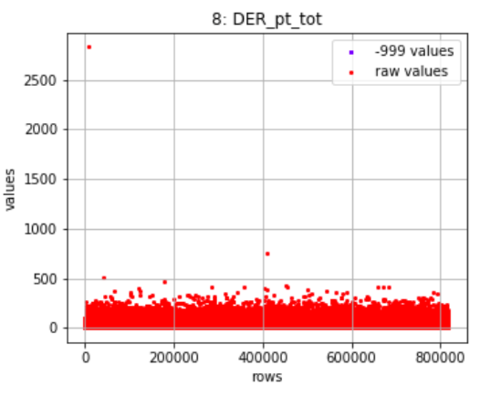
\includegraphics[width=0.77\columnwidth]{outliers}
  \caption{Values of all data items for the DER\_pt\_tot feature. The graph shows a relatively small number of outliers. In this example, all items with values above 400 for this feature were removed.}
  \vspace{-3mm}
  \label{fig:outliers}
\end{figure}


\subsubsection{Distribution Analsysis}
We wanted to see how features values were distributed over both the signal data and the background data. Indeed, we made the assumptions that if two features had a similar distribution between the two sets, then this feature would be independent from the output. Among all features, four were spotted to have the almost exact same distributions between the two labels. Those are "PRI\_tau\_phi", "PRI\_lep\_pt", "PRI\_lep\_phi" and "PRI\_met\_phi". Dropping those columns did not affect the resulting predictions and we inferred that we could do so without losing any meaningful information.

\subsubsection{PRI\_jet\_num-based Split}
After looking further at the data, we noticed that there were a lot of -999 values spread on the dataset. More importantly, we noticed that the amount of those values depended greatly on one particular feature, which happens to be the same categorical feature : "PRI\_jet\_num", representing the number of "jet events" (a physics term unknown to us) occurring at every event. For instance, if this feature has value 0, then 10 other features will have only -999 values and 26\% of the first feature will be -999, as per if it has a value of 3, then no feature is all -999 and only 1.4\% of the first feature will be -999.
We thus chose to split the data into four data subsets depending on the jet number to treat them separately and with more flexibility. We could then safely drop the following features (columns) which did not contain any useful information, i.e. contained a constant value within each set. including the jet number column itself (column 22):

\vspace{1em}
\begin{tabular}{l|l}
\hline
 jet  & columns dropped \\
\hline
0 & [4, 5, 6, 12, 22, 23, 24, 25, 26, 27, 28, 29] \\
1 & [4, 5, 6, 12, 22, 26, 27, 28] \\
2 & [22]  \\
3 & [22]\\
\hline
\end{tabular}
\vspace{1em}


%since it was useless and we need more space, I'll remove it
%\item Correlation Analysis :
%After splitting the data into four subsets we computed the correlations between each pairs of features and tried to drop all but %one of the features in a set of correlated ones. However, we noticed that we obtained a lower ratio of correct predictions. %Therefore, we decided not to drop any of these columns.


\subsubsection{Standardization}
To standardize the data we decided to use the whole dataset to compute the means and standard deviations while carefully not considering the -999 values and hard-coded those values to use them as constants to standardize both sets.

\subsubsection{Percentiles Computation}
A technique we tried and that allowed to increase the ratio of correctly predicted outputs is what we called dimension expansion. We divided each feature in N features using the percentiles. e.g. if N=2 we took the median and split a column into two new columns, one with all the entries below the median and one with all the entries above the median. This allowed to split the dimension of the input in different intervals in which the regression can be trained independently (imagine if you have to fit an exponential with a 1-degree polynomial, you split the input into two intervals and use two 1-degree polynomials instead of 1). Similarly to the standardization, we pre-computed the percentiles and stored them in a file to follow the exact same procedure with the training and testing set. We concatenated to each one of the four datasets its logarithm and noticed that the performance of our model increased. Therefore, we concluded that the output potentially depended logarithmically on some of the features.

%a bit cheesy, might remove it
%With those tools applied to our data, we were ready to actually train our model and find the combination of parameters that would lead to the highest ratio of correct predictions.

\subsection{Algorithms and Techniques}
\subsubsection{Method Selection}
While preparing the data is an important part of any ML system, it only makes sense for specific techniques. 
We thus tried different approaches using the methods presented in class and tested our models by training them with an increasing number of data items and visualized how the performance changed. This allowed to see if the lack of performance came from high bias and/or high variance, thus giving hints about whether we should reduce the number of features or on the contrary, increase it. 
Using the same approach on ridge regression, stochastic gradient descent and logistic regression, it appeared that logistic regression was generally better than the other methods. We thus chose to refine this method and spend more time trying to increase its performance. 

\subsubsection{Hyperparameters Selection}
After several trials we understood that a high polynomial degree did not increase much the ratio of correct predictions and that a 2-degree polynomial was sufficient. Thanks to dimension expansion we could use a simpler polynomial in smaller intervals of each feature, i.e. we split every feature into five intervals, therefore increasing the number of features by a factor of five. Moreover, to each of the four datasets, we concatenated its logarithm (before building the polynomial). These steps were taken in the following order: (1) split the features, (2) compute and concatenate the logarithm of the dataset, (3) build the polynomial.  
We noticed that the higher the degree, the lower was the gamma needed to have a stable gradient descent leading to a higher converging time. Instead of using a scalar gamma we thus used an array of gammas and tuned them independently. In particular, this array of gammas is as long as the gradient of L(w) and allowed us to choose a different step size for different parts of the gradient, yielding a more versatile system. Another solution we tried was to normalize after building the polynomial, but we achieved a higher converging time with the latter therefore we opted for the array of gammas. Note that we decided not to use cross validation with logistic gradient descent because we were using low degree polynomials therefore reducing the variance of our model and we already used cross validation with ridge regression and did not obtained any noticeable overfitting.


\section{Results}
 Since we split our dataset into four groups depending on the jet number, we obtained different precision depending on the group. In total, our model yielded a precision of 84\%, 80\%, 83\% and 82\% on the training set depending on the jet number and resulted on a 83\% precision on the test data according to Kaggle's public leaderboard. Those results allowed us to each the top 20\% of the leaderboard. While not being as high as we hoped, we found those results to be good enough, especially when considering that we started from an ~65\% precision.

\section{Discussion}
Overall, we are satisfied with our results, although it was exponentially more difficult to increase our score and required a lot of work. There are a few techniques given in the course, such as cross-validation and model selection methods, that we tried to use but to no significant avail. Indeed, we did not find any sign of overfitting in our system and thus saw no use of cross-validation.
We could not think of much more to do to increase our score on the data exploration side since we already spent a lot of time on it. Furthermore, we experimented in length with our algorithms without seeing any significant differences in the results and inferred that to reach truly higher precision, we would have to design a completely different method and use other, more complex algorithms. We found this consistent with the fact that we are less than 2\% away from the best results on Kaggle, showing that no other group could achieve something really better than our model. It is true that those few percents make a big difference, but we would expect more advanced methods (e.g. Neural Networks or Decision Trees) to reach at least above the 90\% barrier. 



\bibliographystyle{IEEEtran}
\bibliography{literature}

\end{document}
